% PLEASE FILL IN THE PLACEHOLDERS <...>
%
% Diplomarbeit/Studienarbeit/IDP von <NAME>
% Diploma thesis of <NAME>
%
% Title: <TITLE>
%        <TITLE>
%
\documentclass[12pt,a4paper]{report}

%%%%%%%%%%%%%%%%%%%%%%%%%%%%%%%%%%%%%%%%%%%%%%%%%%%%%%%%%%%%

% PACKAGES:

% Define typearea
% a) Use automatic:
\usepackage[BCOR1cm]{typearea}
% b) Or use fixed: 
%\usepackage{geometry}
%\geometry{left=1.5cm,textwidth=18.5cm,top=1.5cm,textheight=26.5cm}

% Use German :
\usepackage[USenglish]{babel}
% Use list of tabels, etc. in table of contents:
\usepackage{tocbibind}
% German paragraph skip
\usepackage{parskip}
\usepackage{enumitem}
% Encoder:????
%\usepackage[utf-8]{inputenc}
\usepackage[utf8]{inputenc}
% Use A4-paper efficiently:
\usepackage{a4wide}
% Index-generation
\usepackage{makeidx}
% Einbinden von URLs:
\usepackage{url}
% Include .eps-files (needed also for the LKN-logo):
%\usepackage{epsf}
\usepackage{epsfig}
\usepackage{epstopdf}
% Special \LaTex symbols (e.g. \BibTeX):
\usepackage{doc}
% Include Graphic-files:
%\usepackage{graphics}
% Include Graphic-files:
\usepackage{graphicx}
% Include doc++ generated tex-files:
%\usepackage{docxx}
% Include PDF links
%\usepackage[pdftex, bookmarks=true]{hyperref}

\usepackage{amsmath}

%%%%%%%%%%%%%%%%%%%%%%%%%%%%%%%%%%%%%%%%%%%%%%%%%%%%%%%%%%%%

% OTHER SETTINGS:

% Pagestyle:
\pagestyle{headings}

% Avoid 'overhang':
\sloppy

% Choose language
\newcommand{\setlang}[1]{\selectlanguage{#1}\nonfrenchspacing}

%%%%%%%%%%%%%%%%%%%%%%%%%%%%%%%%%%%%%%%%%%%%%%%%%%%%%%%%%%%%

% TITLE:

\begin{document}

\thispagestyle{empty}
\newpage

\vspace{5cm}
\begin{center}
    \epsfxsize=4cm
    \epsfbox{LKN_Logo_klein.eps}
\end{center}

\parbox{15cm}{\begin{center} {\sf\bf 
                               \Large  Technische Universität München
                                \smallskip

                               \Large Lehrstuhl für Kommunikationsnetze
                               \smallskip
                              }

                              {\sf \large Prof. Dr.-Ing. Wolfgang Kellerer} 
              \end{center}}  %&

\vspace{4cm}

\begin{center}
        {\bf\Huge Master‘s Thesis} % Studienarbeit, Interdisziplinäres Projekt
\end{center}

\begin{center}
        \settowidth{\baselineskip}{0.4cm}
        {\LARGE 
        VM Selection Heuristic for Financial Exchanges on the Cloud
        }
\end{center}

\vfill         
{\settowidth{\baselineskip}{0.2cm}
\large\begin{tabular}[l]{ll}
Author: & Duclos-Cavalcanti, Daniel\\
Address: & 230 W 55th Street\\
         & 10019 New York, NY\\
         & U.S.A.\\
Matriculation Number: & 03692475\\
Supervisor: & Muhamadd Haseeb \& Navidreza Asadi\\
Begin: & 03. April 2024\\
End: & 03. October 2024
\end{tabular}}

%%%%%%%%%%%%%%%%%%%%%%%%%%%%%%%%%%%%%%%%%%%%%%%%%%%%%%%%%%%%

% MAIN PART:
% Independence and License statements
\include{Statements}
% German abstract:
\setlang{german}
\thispagestyle{plain}

\section*{Kurzfassung} 
A short abstract of the thesis in German. 
% English abstract:
\setlang{USenglish}
\thispagestyle{plain}

\section*{Abstract}
Financial exchanges consider a migration to the cloud for scalability, robustness, and cost-efficiency.
Jasper presents a scalable and fair multicast solution for cloud-based exchanges, 
addressing the lack of cloud-native mechanisms for such. 
To achieve this, Jasper employs an overlay multicast tree, leveraging clock synchronization, kernel-bypass techniques, 
and more.
However, there are opportunities for enhancement by confronting the issue of inconsistent VM performance 
within identical instances. LemonDrop tackles this problem, detecting under-performing VMs in a cluster 
and selecting a subset of VMs optimized for a given application's latency needs.
Yet, we believe that LemonDrop's approach of using time-expensive all-to-all latency measurements and an optimization routine 
for the framed Quadratic Assignment Problem (QAP) is overly complex. 
The proposed work aims to develop a simpler and scalable heuristic, that achieves reasonably good results
within Jasper's time constraints. 



% Table of contents:
\tableofcontents  
% Introduction (Einleitung):
\chapter{Introduction}

This chapter should give a short overview over the whole thesis. It should provide background information on the thesis topic, introduce the task definition and give a short outlook on the rest of the thesis. 


% Text Body (Hauptteil)
% Could have multiple chaper-files, e.g.:
\chapter{Background}

\section{Content}
In this chapter, all background necessary to understand the thesis are introduced. The level of detail is such that a colleague with similar background (no specialist!) is capable of understanding the contribution and impact of the thesis. A discussion of state-of-the-art solutions (e.g. literature research) is often helpful. Problems of the state-of-the-art are typically discussed and the contribution of the thesis is introduced in detail. 

\chapter{Implementation/Results}
\section{Implementation}
Details regarding implementation and/or simulation are given in this chapter. The considered setup and the parameters used are introduced and discussed. Also, the general evaluation methods can be presented. (Note: Code should not be part of this chapter. If it makes sense to introduce it into the thesis, it should be placed in the appendix.)

\section{Results}
Results of the performed investigations are presented here. Interpretations for the observed effects are given and the impact of investigations is discussed. 

%  Conclusions (Zusammenfassung):
\chapter{Conclusions and Outlook}

The thesis is concluded here. The considered problem is repeated. The contribution of this work is highlighted and the results are recapitulated. Remaining questions are stated and ideas for future work are expressed. 
%\chapter{Formatting}

\section{Figures and Tables}
Figures and tables need to include a caption. This can be done with the LaTeX-command \texttt{\bslash caption$\lbrace\rbrace$}. To be able to reference figures and tables, a \texttt{\bslash label$\lbrace\rbrace$} must follow the caption.

\begin{figure}[h!]
  \begin{center}
    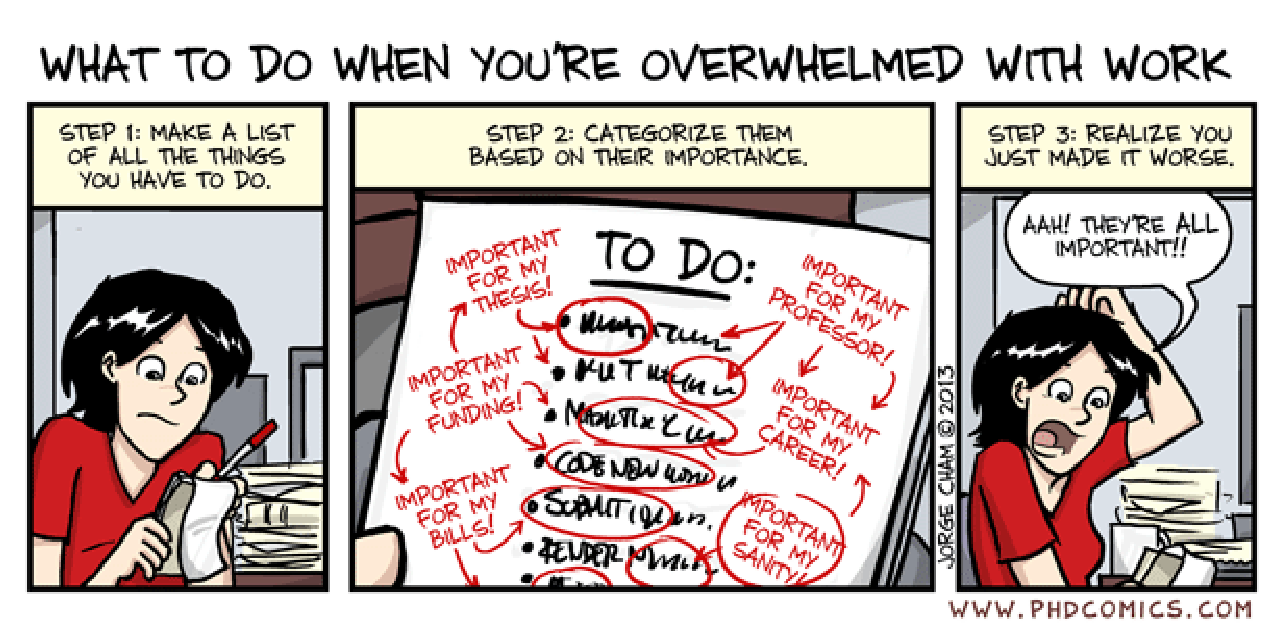
\includegraphics[width=0.6\textwidth]{phd112013s.eps}
    \caption{Ein PHD Comic}
    \label{fig:ToUseWithReference}
  \end{center}
\end{figure}

\begin{table}[b]
\begin{center}
\begin{tabular}{|l |c|}
\hline 
\textbf{Parameter} & \textbf{Value} \\
\hline  
\hline 
Transmission Power & 23~dBm\\
\hline 
Center Frequency & 2.6~GHz\\
\hline 
Channel Bandwidth & 15~kHz\\
\hline 
Shadowing Correlation Distance & 40~m\\
\hline 
Noise Density & -174~dBm/Hz\\
\hline 
Antenna Heights & 1.5~m\\
\hline 
\end{tabular}
\caption{Simulation Parameters and Values}\label{tab:param_table}
\end{center}
\end{table}

The labelled figures and tables can be referenced via \texttt{\bslash ref}, e.g. ~Figure~\ref{fig:ToUseWithReference}.
\newpage

\section{Referencing}
Literature references are included e.g. like this:\\
``..., as shown in \cite{eberspaecher97},, ...'' or ``... there are several approaches \cite{arnaud99,griswold90} ...''

% Appendix (Anhänge), could have multiple chaper-files:
\appendix
\chapter{}
The appendix may contain some listings of source code that has been used for simulations, extensive proofs or any other things that are strongly related to the thesis but not of immediate interest to the reader. 

% Abbreviations (Abkürzungsverzeichnis):
\chapter{Abbreviations}
\begin{table}[h]
\begin{tabular}{ll}
CES & Central Exchange Server \label{abbr:CES}\\
MP & Market Participant \label{abbr:MP}\\
VM & Virtual Machine \label{abbr:VM}\\
\end{tabular}
\end{table}




% References (Literaturverzeichnis):
% a) Style (with numbers: use unsrt):
\bibliographystyle{alpha}
% b) The File:
\bibliography{Bibliography}


%%%%%%%%%%%%%%%%%%%%%%%%%%%%%%%%%%%%%%%%%%%%%%%%%%%%%%%%%%%%


%%%%%%%%%%%%%%%%%%%%%%%%%%%%%%%%%%%%%%%%%%%%%%%%%%%%%%%%%%%%


%%%%%%%%%%%%%%%%%%%%%%%%%%%%%%%%%%%%%%%%%%%%%%%%%%%%%%%%%%%%
\end{document}
